\documentclass[11pt]{article}
\usepackage[margin=1in]{geometry}
\usepackage{amsmath,amssymb}
\usepackage{graphicx}
\usepackage{booktabs}
\usepackage{hyperref}
\usepackage{xcolor}
\usepackage{caption}
\hypersetup{colorlinks=true, linkcolor=blue, urlcolor=blue, citecolor=blue}

\title{Same Referee, Different Games: Cross-Cube Evidence of Systematic\\
Pipeline Bias in Simulated \emph{Magic: The Gathering} Drafts}

\author{
  \textit{[Your name here]} \\
  \small Independent cube design research
}
\date{August 2026}

\begin{document}
\maketitle

\begin{abstract}
Bot-draft-and-simulate pipelines -- pairing an automated drafting bot with an
automated match engine -- are an increasingly practical way to generate
empirical, data-driven signal about a cube's balance at a scale no human
playtesting group can match. But such a pipeline is itself an instrument, not a
neutral referee: if any of its stages carries a systematic bias, a single-cube
study has no way to distinguish ``this cube is unbalanced'' from ``this
instrument has its own opinions.''

We test whether that concern is real by running one such pipeline (CubeCobra bot
drafting and deck construction, Forge headless match simulation) against five
independently designed, publicly available CubeCobra cubes spanning nearly the
full power-level spectrum used in cube drafting -- from an all-commons Pauper
cube to the Power-9-inclusive MTGO Vintage Cube. A mono-color win-rate premium
appears in all five, positive in direction throughout ($+5.7$ to $+13.7$
percentage points at the draft level) and reaching conventional statistical
significance in three of the five when tested at the more conservative
draft-paired level. A second, more specific
pattern also recurs in all five: whatever mechanic in a given cube's card pool
requires the most sequential, precisely-timed planning to pay off -- cantrip-based
card selection in two cubes, a full storm-combo package in one,
artifact-ramp-into-expensive-threats in two -- has by far the lowest win rate in
that cube, while efficient, low-commitment aggressive strategies dominate
regardless of which specific cube is tested. As a further, more tentative
observation, two of the five cubes happen to both include genuine cards with the
always-on evasion keyword Shadow, despite no other overlap in card pool or
design philosophy, and those cards outperform their own cube's mono-color
baseline in both. We conclude that a meaningful share of the card-level
performance signal produced by this pipeline is systematic across cubes, rather
than attributable to any individual cube's design alone -- while explicitly
flagging that this study cannot yet localize
that property to drafting, deck construction, or match play specifically.
\end{abstract}

\section{Introduction}

Cube designers increasingly have access to a genuinely useful empirical tool:
pairing an automated drafting simulator with an automated match engine to
generate large volumes of played-out games without needing a human playtest
group. This makes data-driven cube design possible at a scale that was previously
impractical -- hundreds of drafts and thousands of matches can be generated and
analyzed in a single session.

But this approach rests on an assumption worth checking explicitly: that the
pipeline's output reflects the cube's actual balance and nothing else. Such a
pipeline has several stages -- an automated bot decides what to draft and how to
build a deck from it, then an automated engine plays that deck out against
others -- and any one of those stages could carry its own systematic bias,
independent of what any particular card pool contains. A designer running this
kind of pipeline on their own cube alone has no way to tell ``my card pool is
unbalanced'' apart from ``one stage of this pipeline has its own opinions.''

This paper tests that concern directly. We ran a bot-draft-and-simulate pipeline
against five cubes, chosen deliberately for two properties: they are
independently designed by different people with different goals and philosophies,
and they are among the most-used cubes on CubeCobra, so any pattern found here is
informative to a far larger audience than any single custom cube would be. If the
same directional patterns turn up across five cubes that share essentially
nothing -- different card pools, different power levels, different design
intentions -- the most natural common factor to investigate is the one thing
they were all run through: the pipeline itself. We deliberately do not claim to
know \emph{which} stage of the pipeline produces the effects reported below;
\S4 discusses why that
question is left open, and what would be needed to answer it.

\section{Methods}

\subsection{Cube selection}

\begin{table}[h]
\centering
\caption{The five cubes tested, spanning the power-level range used in cube
drafting. All are public CubeCobra cubes; card pools and archetype labels are each
cube's own, unmodified.}
\begin{tabular}{lp{9cm}}
\toprule
Cube & Notes \\
\midrule
The Pauper Cube & Commons only; the lowest power level tested. \\
World Championship Museum (96-04) & Built exclusively from cards that appeared in
official World Championship decks, 1996--2004. \\
The 2017 Classic Modern Cube & Modern-legal power level. \\
The Peasant Cube 2026 & Commons and uncommons. \\
MTGO Vintage Cube & Wizards' official Vintage-format cube; includes the Power 9
and other Reserved List cards. The highest power level tested. \\
\bottomrule
\end{tabular}
\end{table}

Cubes were selected for design independence (different curators, no shared
lineage) and for being among CubeCobra's highly drafted lists, so that this
study concerns cube lists of practical relevance to existing CubeCobra users --
we make no claim that five cubes constitute a representative sample of that
user base, only that they are not an arbitrary or convenient one.

\subsection{Pipeline stages}

Each cube was drafted 50 times (400 decks) using CubeCobra's bot-drafting
simulator. Critically, \emph{deck construction is also performed by this same
bot} during the draft -- CubeCobra's drafting bot decides both what to pick and
how to build its final maindeck/sideboard split, and this decision is exported
directly as part of the draft record. Our pipeline converts that record verbatim
into Forge's \texttt{.dck} deck format: Forge is never asked to build a deck from
a larger pool, and has no deck-construction role in this study. Forge's only
function here is playing pre-built decks against each other in a best-of-one,
8-seat round-robin (28 matches per draft, 1{,}400 matches per cube, 7{,}000
matches total across the five).

This matters for interpretation: the ``pipeline'' whose output we study bundles
(a) CubeCobra's bot-drafting policy, (b) CubeCobra's bot deck-construction policy,
and (c) Forge's match-play policy into a single measurement. All results below
should be read as properties of this bundle, not as isolated to any one stage --
see \S4.1 for why we did not attempt to separate them in this study.

\subsection{Operational definitions}

A deck is classified as \emph{mono-color} if its CubeCobra-assigned archetype
label resolves to exactly one color letter (e.g. \texttt{W\_Weenie}) and
\emph{multi-color} if it resolves to two or more (e.g. \texttt{RW\_Aggro});
archetype labels that do not resolve to a recognizable color prefix (e.g. a
generic \texttt{Combo} label) are excluded from this classification rather than
forced into either bucket.

A card's reported win rate is the pooled win rate of every deck that included
it in its 40-card list for that match, \emph{not} a rate conditioned on the card
having actually been drawn, cast, or resolved in that game. This is a
deliberate, necessary simplification -- individual card-cast events are not
tracked at that granularity by this pipeline -- but it means a card's reported
win rate should be read as ``how decks containing this card performed'' rather
than as an estimate of that card's marginal, in-game impact. This distinction
matters most for \S3.2: a card's win rate under this definition can be low
either because it performs poorly when drawn, or because it tends to end up in
decks that perform poorly for other reasons (an incomplete combo shell, for
instance), and this paper's data cannot separate the two.

A card is treated as \emph{reliable} for win-rate reporting once it has
appeared in at least two distinct drafts within a cube's 50-draft corpus, to
avoid the case where a card seen in only one deck mechanically inherits that
deck's overall win/loss record rather than providing an independent signal;
Tables~\ref{tab:spread} and \ref{tab:shadow} report only reliable cards. We
checked this threshold's effect on \S3.2's results by recomputing
Table~\ref{tab:spread} at $\geq 5$ and $\geq 10$ distinct drafts instead of
$\geq 2$: the top-15/bottom-15 averages shift by at most 2 percentage points
in any cube, and by nothing at all in three of the five, so the pattern
reported there is not an artifact of the more permissive threshold used in the
main tables. The ``bottom-15 characterized by'' column in
Table~\ref{tab:spread} reflects the authors' manual, qualitative reading of what
those fifteen cards have in common, produced after observing the ranking -- it is
an exploratory characterization, not a pre-defined or quantified category (see
\S4.4).

\subsection{Guardrails}

Two measurement guardrails were established and validated before this study,
against manual inspection of raw match logs. First, win detection is anchored to
the single, unambiguous \texttt{Match Winner -} log line rather than
pattern-matching narrative outcome text, which is vulnerable to AI turn-timeouts
emitting contradictory outcome lines for the same game. Second, the legal
blocking rate (used only in supporting analysis, not in the results reported
here) is computed from a reconstructed board state rather than a naive count of
``didn't block'' lines, which conflates an empty board, a legally-unblockable
attacker, and a genuine missed block. No card list, keyword list, or analysis
parameter was adjusted for any individual cube tested here.

\subsection{Statistical tests}

The primary test for \S3.1 is a one-sample, two-tailed $t$-test and a Wilcoxon
signed-rank test (both against $H_0: \Delta=0$) on the per-draft
$\Delta = WR_{\text{mono}} - WR_{\text{multi}}$ values within each cube; 95\%
confidence intervals on the mean use the $t$-distribution. The pooled
match-level comparison in Table~\ref{tab:monogap} uses a 2-proportion
$z$-test, reported for continuity with an earlier version of this analysis and
discussed critically in \S3.1 and \S4.3 rather than treated as primary evidence.

\subsection{Software versions}

All matches were played using Forge 2.0.14 (\texttt{forge-installer-2.0.14}).
All five cubes' draft data was exported from CubeCobra's bot-drafting simulator
on 15 August 2026; any changes to CubeCobra's bot-drafting policy after that date
are not reflected in this study.

\section{Results}

\subsection{A mono-color premium, confirmed at the draft level in three of five cubes}

The primary test of the mono-color premium reported here is a draft-level paired
comparison: for each draft, $\Delta = WR_{\text{mono}} - WR_{\text{multi}}$ (the
pooled mono-color win rate minus the pooled multi-color win rate within that one
draft), giving up to 50 approximately independent observations per cube rather
than 1{,}400 non-independent match outcomes. Drafts with zero mono-color or zero
multi-color decks (no basis for a within-draft comparison) are excluded; this
was rare in four of the five cubes but notable in the MTGO Vintage Cube, where 16
of 50 drafts (32\%) had no directly comparable mono-color deck, itself an
observation about that cube's drafting environment worth noting in passing.

\begin{table}[h]
\centering
\caption{Draft-level paired comparison, $\Delta = WR_{\text{mono}} -
WR_{\text{multi}}$ per draft. One-sample $t$-test and Wilcoxon signed-rank test
against $H_0: \Delta = 0$; 95\% CI on the mean via the $t$-distribution.}
\label{tab:draftlevel}
\footnotesize
\begin{tabular}{lrrrrrr}
\toprule
Cube & $n$ drafts & Mean $\Delta$ & 95\% CI & \% drafts $>0$ & $t$-test $p$ & Wilcoxon $p$ \\
\midrule
The Pauper Cube & 49 & +13.66 & [8.31, 19.02] & 75.5\% & $5.2\times10^{-6}$ & $2.5\times10^{-5}$ \\
World Championship Museum & 49 & +7.97 & [1.98, 13.97] & 59.2\% & $1.0\times10^{-2}$ & $8.3\times10^{-3}$ \\
The 2017 Classic Modern Cube & 47 & +8.56 & [3.14, 13.98] & 66.0\% & $2.6\times10^{-3}$ & $1.6\times10^{-3}$ \\
The Peasant Cube 2026 & 48 & +5.68 & [$-$0.87, 12.24] & 58.3\% & $8.8\times10^{-2}$ & $8.7\times10^{-2}$ \\
MTGO Vintage Cube & 34 & +7.45 & [$-$1.13, 16.03] & 64.7\% & $8.7\times10^{-2}$ & $9.1\times10^{-2}$ \\
\bottomrule
\end{tabular}
\end{table}

At this more conservative unit of analysis, the point estimate is positive in
all five cubes, and reaches conventional significance ($p<0.05$, both tests
agreeing closely) in three: the Pauper Cube, World Championship Museum, and the
2017 Classic Modern Cube. In the remaining two -- the Peasant Cube 2026 and the
MTGO Vintage Cube -- the 95\% confidence interval crosses zero, and a majority of
individual drafts still favor mono-color (58\% and 65\% respectively), but the
result does not reach significance at this sample size. We report this
honestly as a weaker and more mixed result than the pooled match-level test
below suggests, rather than treating the three significant cubes as
representative of all five.

For comparison, and because it was our original (less rigorous) test, the pooled
match-level result is reproduced in Table~\ref{tab:monogap}. It agrees in
direction with Table~\ref{tab:draftlevel} in every cube, but its 2-proportion
$z$-test treats each match as an independent observation, which \S4.3 discusses
in more detail; we no longer treat its $p$-values as the primary evidence for
this finding; and this discrepancy from the previous version of this analysis
is itself the reason we no longer do so.

\begin{table}[h]
\centering
\caption{Pooled mono- vs.\ multi-color win rate, all five cubes (match-level,
non-independent observations -- see discussion above and \S4.3).}
\label{tab:monogap}
\small
\begin{tabular}{lrrrrr}
\toprule
Cube & Mono WR & Multi WR & Gap (pts) & $z$ & $p$ \\
\midrule
The Pauper Cube & 56.90\% & 44.69\% & +12.21 & 6.40 & $1.5\times10^{-10}$ \\
World Championship Museum & 53.91\% & 46.32\% & +7.59 & 3.98 & $6.9\times10^{-5}$ \\
The 2017 Classic Modern Cube & 55.48\% & 47.76\% & +7.72 & 3.81 & $1.4\times10^{-4}$ \\
The Peasant Cube 2026 & 54.98\% & 48.36\% & +6.62 & 3.02 & $2.5\times10^{-3}$ \\
MTGO Vintage Cube & 55.43\% & 49.22\% & +6.20 & 2.17 & $3.0\times10^{-2}$ \\
\bottomrule
\end{tabular}
\end{table}

Three of five individually significant leaves open a natural question: is the
effect itself, combined across all five independently designed cubes,
distinguishable from zero? A fixed-effect, inverse-variance-weighted
meta-analysis of the five per-cube estimates in Table~\ref{tab:draftlevel}
answers this directly: pooled $\Delta = +9.15$ points, $\text{SE}=1.36$, 95\% CI
$[6.49, 11.81]$, $z=6.74$, $p=1.6\times10^{-11}$. A random-effects
(DerSimonian--Laird) version of the same meta-analysis, run as a sensitivity
check on the fixed-effect assumption, gives an almost identical estimate
($\Delta=+9.11$, SE$=1.43$, 95\% CI $[6.32, 11.90]$, $p=1.7\times10^{-10}$),
which is reassuring but not dispositive given only five studies to estimate
between-cube variance from. A Cochran's $Q$ test for heterogeneity across the
five cube-level estimates does not reject homogeneity ($Q=4.37$, $df=4$,
$p=0.36$); we read this as finding no evidence of substantial heterogeneity
among the five estimates, rather than as evidence that the five cubes' true
effect sizes are identical -- with only five studies, $Q$ has limited power to
detect real between-cube differences, and a non-significant result should not
be over-interpreted as confirming homogeneity. Figure~\ref{fig:forest} shows
all five estimates and the fixed-effect pooled result together.

\begin{figure}[h]
\centering
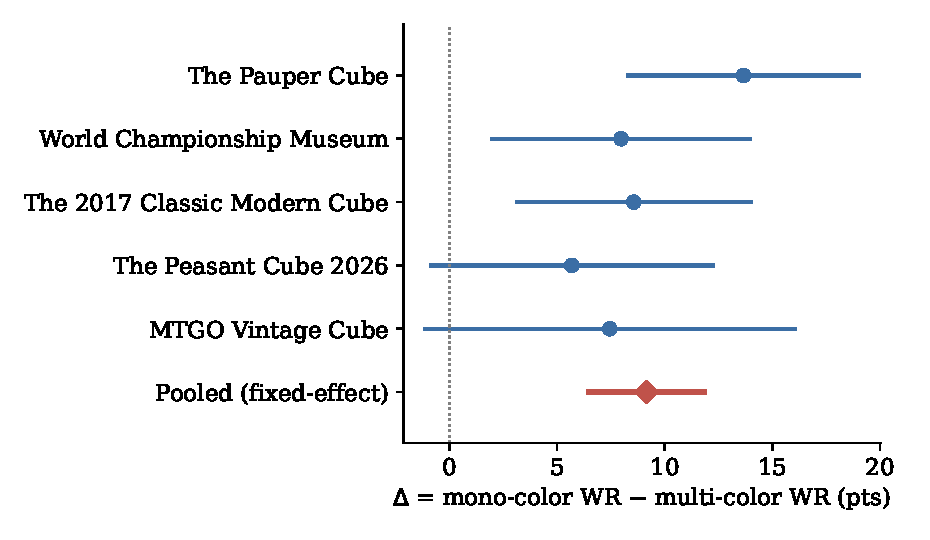
\includegraphics[width=0.62\textwidth]{fig_forest.pdf}
\caption{Draft-level $\Delta$ (mono-color WR $-$ multi-color WR) per cube, 95\%
CI, and the fixed-effect pooled estimate across all five.}
\label{fig:forest}
\end{figure}

The overall picture we take from this section: a mono-color premium of roughly
$6$--$14$ percentage points at the individual-cube level, positive in direction
in every cube tested, statistically robust to a conservative draft-level test in
three of five individually, and -- combined across all five via meta-analysis --
clearly distinguishable from zero as a pooled effect even though two individual
cubes did not reach significance alone. This is a more careful claim than
``every cube shows a significant premium,'' and we think it is the correct one
to make; it is also, we think, a stronger one, since it does not depend on
treating five moderate-sample estimates as if each had to clear a significance
bar independently before the combined evidence could be taken seriously.

\subsection{A complexity gradient: simple plans overperform, multi-step plans underperform}

\begin{table}[h]
\centering
\caption{Mean win rate of each cube's 15 best- and 15 worst-performing reliable
cards, and what mechanically characterizes the bottom 15 (author's qualitative
reading -- see \S2.3).}
\label{tab:spread}
\small
\begin{tabular}{lrrrp{4.3cm}}
\toprule
Cube & Top-15 avg & Bottom-15 avg & Spread & Bottom-15 characterized by \\
\midrule
World Championship Museum & 85.59\% & 23.15\% & 62.44pt & Cantrips \& counterspells (Brainstorm, Opt, Serum Visions, Undermine, Mystical Tutor) \\
MTGO Vintage Cube & 74.38\% & 17.87\% & 56.51pt & A near-complete storm-combo package (Dark Ritual, Doomsday, Tendrils of Agony, Yawgmoth's Will, Underworld Breach) \\
The 2017 Classic Modern Cube & 73.77\% & 24.60\% & 49.17pt & Artifact mana rocks \& expensive colorless threats (Chromatic Sphere/Star, Hedron Archive, Blightsteel Colossus) \\
The Peasant Cube 2026 & 71.31\% & 27.18\% & 44.14pt & Graveyard reanimation \& artifact ramp (Animate Dead, Exhume, Reanimate, Everflowing Chalice) \\
The Pauper Cube & 69.79\% & 30.53\% & 39.26pt & Cantrips (Preordain, Behold the Multiverse, Growth Spiral, Capsize) \\
\bottomrule
\end{tabular}
\end{table}

This is an exploratory finding, not a confirmatory one, and we present it as
such. The ``bottom 15'' in each cube was identified purely by observed win rate;
the characterization of what those cards have in common (cantrips, combo pieces,
ramp) was produced afterward, by inspection, not from a pre-defined or quantified
complexity measure. Selecting extreme performers from a ranked list of hundreds
of cards and then noticing a shared property is a standard and legitimate way to
generate a hypothesis, but it is not yet a test of one -- a reliability threshold
of two distinct drafts (\S2.3) is a meaningful floor against single-deck noise,
but is weak enough that some cards in these tables may still reflect small-sample
variance rather than the pattern described below.

With that caveat, the pattern is nonetheless consistent across all five cubes:
the specific mechanic occupying the bottom of each cube's card pool differs --
unsurprisingly, since several of these mechanics (a full storm combo, artifact
mana rocks) do not exist in every cube tested -- but the \emph{kind} of mechanic
that ends up there does not. In every one of the five cubes, without exception,
the worst-performing cluster is a strategy that only pays off after several
correctly-sequenced, precisely-timed steps, while efficient, low-commitment
creatures with an immediate board impact occupy the top of every cube's list
instead, regardless of that cube's power level or design philosophy (Figure~\ref{fig:spread}).
The severity of the pattern also scales sensibly with how demanding each cube's
available multi-step strategies are: the MTGO Vintage Cube and World
Championship Museum show the widest top-to-bottom spreads ($56$--$62$ points),
while the Pauper Cube, which lacks true combo pieces, shows the narrowest
($39$ points) while still following the same direction. We treat this as a
hypothesis worth a dedicated, quantified follow-up (\S4.4) rather than as
established here.

\begin{figure}[h]
\centering
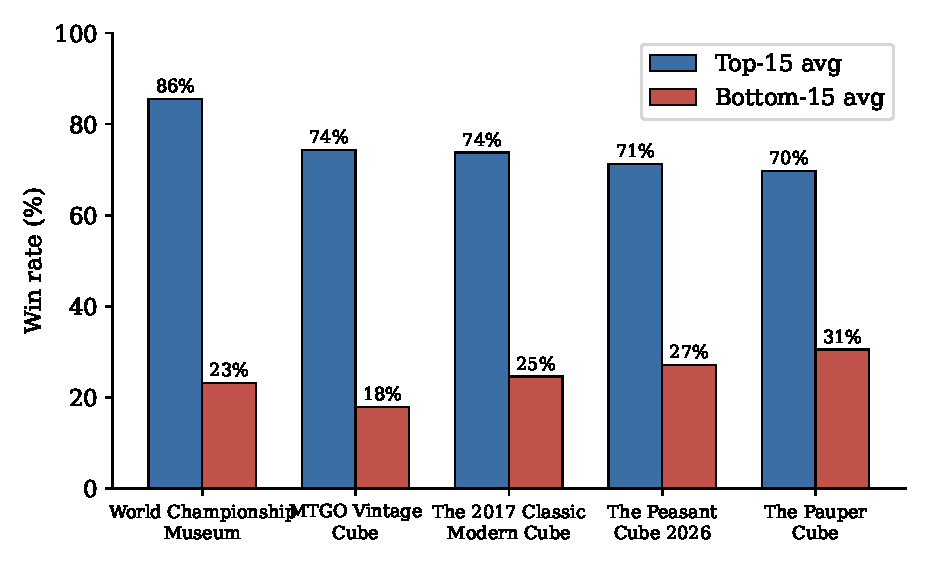
\includegraphics[width=0.62\textwidth]{fig_spread.pdf}
\caption{Top-15 vs.\ bottom-15 average reliable-card win rate, per cube.}
\label{fig:spread}
\end{figure}

The same pipeline-stage confounding discussed for \S3.1 in \S4.1 applies here,
and arguably more so: a bottom-15 cluster's low win rate could reflect Forge's
match-play policy struggling to execute a multi-step plan, or it could equally
reflect CubeCobra's drafting/deck-construction bot failing to assemble a
sufficiently coherent version of that plan in the first place (an incomplete
storm package, a reanimation shell missing its enablers). Nothing in this
section's data distinguishes ``the AI plays combo badly'' from ``the bot
doesn't draft combo well enough to play,'' and we do not intend the phrase
``complexity gradient'' to imply we have.

\subsection{Exploratory observation: the evasion keyword Shadow outperforms in two independently designed cubes}

Two of the five cubes tested happen to include genuine creatures with the
keyword \emph{Shadow} (a static evasion ability under which the affected creature
can be blocked only by other Shadow creatures) -- the Pauper Cube and World
Championship Museum. This is incidental to cube selection: the two cubes share
essentially no other design overlap, sit at very different power levels, and were
curated by different people.

\begin{table}[h]
\centering
\caption{Win rate of every reliable Shadow-keyword card found across the five
cubes tested.}
\label{tab:shadow}
\small
\begin{tabular}{llrrr}
\toprule
Cube & Card & Win rate & Matches & Distinct drafts \\
\midrule
The Pauper Cube & Dauthi Slayer & 64.76\% & 105 & 15 \\
The Pauper Cube & Soltari Trooper & 62.34\% & 77 & 11 \\
The Pauper Cube & Dauthi Horror & 52.68\% & 112 & 16 \\
World Championship Museum & Soltari Visionary & 74.29\% & 35 & 5 \\
World Championship Museum & Soltari Monk & 71.43\% & 28 & 4 \\
World Championship Museum & Soltari Priest & 71.43\% & 42 & 6 \\
\bottomrule
\end{tabular}
\end{table}

Pooled across each cube's three cards, Shadow averages $59.9\%$ in the Pauper
Cube (against that cube's own $56.9\%$ mono-color baseline) and $72.4\%$ in World
Championship Museum (against that cube's own $53.9\%$ mono-color baseline). We
flag this explicitly as the most tentative finding in this paper: two cubes is a
small basis for any general claim about a specific keyword, sample sizes per card
are modest (4--16 distinct drafts), and we did not pre-specify Shadow as a
mechanic of interest before observing these cubes' card pools. We report it as an
exploratory observation consistent with the complexity-gradient finding above --
an always-on evasion ability requiring no activation or sequencing sits at the
opposite end of the spectrum from \S3.2's worst performers -- and as a candidate
for confirmatory follow-up in a cube that includes it deliberately, not as a
result this paper treats as established.

\section{Discussion}

\subsection{What this study does and does not isolate}

The central limitation of this study, stated plainly: \textbf{it cannot
distinguish a bias originating in the drafting bot's card evaluation, the same
bot's deck-construction logic, or Forge's match-play policy.} All three are
bundled into every result reported above, constant across all five cubes tested.
It is entirely possible that CubeCobra's bot simply drafts and builds better
mono-color decks -- tighter curves, more consistent mana, fewer speculative
picks -- and that Forge's match-play engine is comparatively neutral; it is
equally possible that deck construction is unbiased and Forge's play policy
favors simple game plans; either explanation, or some mixture of both, is
compatible with the data reported here. This
paper establishes that a large, consistent, direction-stable effect is observed
under this shared pipeline across independently designed cubes; it does not
establish that the pipeline causes that effect in any one of its specific
stages, nor which stage would be responsible if it does.

Isolating the source would require a factorial design: holding the drafted card
pool fixed while varying the deck-construction policy, and holding decks fixed
while varying the match-play engine, then checking whether the effect tracks the
drafting/deckbuilding stage, the match-play stage, or persists regardless. We
did not attempt this here and present it as the natural next study.

\subsection{A caution for cube designers using automated pipelines}

A bot-draft-and-simulate pipeline is a genuinely useful tool for data-driven cube
design, and nothing in this paper argues otherwise. But these results show that
such a pipeline measures at least two things at once: the cube's actual design,
and systematic properties of the pipeline used to evaluate it. A single-cube
study cannot cleanly separate the two without a point of comparison outside that
one cube. A designer seeing their combo package or their card-selection spells
underperform in simulation should weigh the possibility that the pipeline, not
the card, is the limiting factor -- particularly if the underperforming strategy
requires several correctly-sequenced steps to pay off, which is precisely the
pattern found here in five independently designed cubes.

\subsection{Limitations}

\textbf{Pipeline-stage confounding.} As discussed in \S4.1, this study cannot
determine whether observed effects originate in drafting, deck construction, or
match simulation.

\textbf{Non-independence of observations.} Matches generated from the same draft
share decks and are therefore not statistically independent; Table~\ref{tab:monogap}'s
$p$-values should be read as suggestive rather than confirmatory. We addressed
this directly with the draft-level paired test in Table~\ref{tab:draftlevel},
which is why that table, not Table~\ref{tab:monogap}, is this paper's primary
evidence for \S3.1 -- and why that more conservative test's weaker result in two
of the five cubes should be taken at face value rather than explained away.

\textbf{Post-hoc characterization.} The complexity-gradient finding (\S3.2) was
identified by inspecting results, not by testing a pre-defined, quantified
hypothesis, and should be treated as exploratory.

\textbf{Multiple comparisons.} This paper reports several analyses over the same
five-cube dataset without correcting for multiple comparisons; card-level
findings in particular should not be read as confirmatory without independent
replication.

\textbf{Format.} All matches are best-of-one: no card ever moves between a
maindeck and a sideboard mid-match, so a card that only earns its keep in a
specific matchup is played every game regardless of opponent if maindecked. This
could inflate the measured gap in \S3.2 beyond what a format with real sideboard
access would show; we do not have data here to estimate that effect's size.

\textbf{Scope.} These results describe one specific software pipeline's behavior
on five card pools at one point in time; they are not a claim about human play,
about any other simulation engine, or about how these cubes perform at an actual
table.

\subsection{Future work}

Two follow-ups would meaningfully strengthen this line of inquiry -- beyond the
draft-level reanalysis already incorporated into \S3.1 above. First, the
factorial design outlined in \S4.1 -- varying the
deck-construction and match-play stages independently -- would localize the
effects reported here to a specific pipeline stage rather than the pipeline as a
whole. Second, a pre-registered, quantified complexity score (e.g. number of
prerequisite cards, timing-sensitive interactions, or required resources for a
strategy to function) tested directly against win rate via regression would
convert \S3.2 from a hypothesis-generating observation into a confirmatory test.

\section{Conclusion}

Running a bot-draft-and-simulate pipeline against five independently designed
public cubes -- spanning the power range from all-commons Pauper to Power-9
Vintage -- reveals two directional patterns that recur across all five. A mono-color
win-rate premium is positive in all five and, under a conservative draft-level
paired test, statistically significant in three; the remaining two show the same
direction (a majority of individual drafts favor mono-color) without reaching
significance at this sample size, and we report that split honestly rather than
rounding it up to ``significant everywhere.'' A much larger, more consistent gap
between simple, low-commitment strategies and multi-step ones recurs without
exception in all five, regardless of which specific mechanic occupies each end of
that spectrum in a given cube. A more tentative, exploratory observation adds
that where the evasion keyword Shadow happens to exist in two of the five,
independently designed and otherwise unrelated, its cards outperform their own
cube's mono-color baseline in both. Taken together, this indicates that a
meaningful share of the card-level performance signal produced by this
pipeline is systematic across cubes, rather than attributable to any
individual cube's design alone. This study does not
isolate which pipeline stage produces that property, and treats doing so as the
natural next step -- but the practical implication for cube designers holds
regardless of that open question: a bot-draft-and-simulate pipeline should be
treated as an instrument that may need calibration, not as a neutral measurement
of a cube's balance.

\section*{Data and Code Availability}
All raw simulation logs, exported draft records (\texttt{cards.csv},
\texttt{SUMMARY.md}, \texttt{analysis.json}), and the pipeline scripts used to
produce every number in this paper are available at
\textit{[GitHub repository URL to be added here]}. All statistics reported here
were computed directly from those files by the scripts in that repository; none
were transcribed or re-derived by hand.

\section*{References}
\begin{enumerate}
\item CubeCobra. \url{https://cubecobra.com}. Bot-drafting simulator used to
generate all draft data in this study.
\item Forge (Card Forge project). Open-source \emph{Magic: The Gathering} rules
engine, version 2.0.14. \url{https://github.com/Card-Forge/forge}.
\end{enumerate}

\section*{Acknowledgments}
All numerical results in this paper were independently recomputed from each
cube's raw \texttt{cards.csv} / \texttt{SUMMARY.md} export files. Cube selection
was guided by CubeCobra's own popularity and power-level categorization; card
pools, archetype labels, and draft outcomes are each cube curator's own and were
not altered in any way for this study. Pipeline development and analysis were
conducted through an iterative, multi-assistant process, including critical
review of an earlier draft of this manuscript by multiple independent reviewers.

\end{document}
